\documentclass[a4paper]{article}

\usepackage{pdp}

%------------------------------------------------------------------------------
%	REPORT INFORMATION
%------------------------------------------------------------------------------

\title{Checkers -- Java}
\subtitle{Rapport final}
\author{RANDRIAMIHAJA Lalatiana, RAMANANAHERISOA Fy-Tommy, HOAREAU Faniry, ATWI Daniel, RAZAFINDRAKOTO Sarah}

%------------------------------------------------------------------------------

\begin{document}

%------------------------------------------------------------------------------
%	TITLE PAGE
%------------------------------------------------------------------------------

\maketitle
\thispagestyle{empty}

%------------------------------------------------------------------------------
%	MAIN MATTER
%------------------------------------------------------------------------------

\section*{Introduction}

\section{Contexte et objectifs du projet}

Le projet a pour objectif de concevoir et développer un logiciel permettant de jouer au jeu de
dames conformément aux règles officielles. Le programme doit permettre à deux joueurs de
s'affronter sur un damier, soit en mode local, soit à distance via un réseau.

Le logiciel garantit le respect strict des règles du jeu tout en proposant une expérience
utilisateur claire, robuste et extensible. Il s'inscrit dans une démarche de développement
logiciel complète, intégrant la qualité du code, la documentation, les tests et les performances.

\subsection{Variantes supportées}

Le jeu de dames se décline en plusieurs variantes internationales, que le programme supporte via
une option de configuration du plateau :

\begin{itemize}
    \item \textbf{Draughts} (style anglo-saxon) : plateau de $8 \times 8$ ;
    \item \textbf{Jeu de dames international} : plateau de $10 \times 10$, chaque joueur disposant
    de 20 pions ;
    \item \textbf{Dames canadiennes} : plateau de $12 \times 12$.
\end{itemize}

\subsection{Règles du jeu}

\subsubsection{Mise en place et déroulement}

Le damier est orienté avec une case foncée en bas à gauche. Les pions se placent exclusivement
sur les cases foncées des quatre premières rangées de chaque camp. Les joueurs jouent chacun à
leur tour ; les blancs commencent toujours.

\subsubsection{Déplacements}

\begin{itemize}
    \item Un \textbf{pion} se déplace d'une case vers l'avant en diagonale.
    \item Un pion atteignant la dernière rangée adverse et s'y arrêtant est promu en
    \textbf{dame} : un point jaune s'ajoute à celui-ci.
    \item Une \textbf{dame} se déplace librement sur une même diagonale, d'autant de cases
    qu'elle le souhaite, en avant comme en arrière.
\end{itemize}

% TODO: insérer figure du plateau de jeu

\subsubsection{La prise par un pion}
\label{sec:prise-pion}

Un pion capture un pion adverse en sautant par-dessus lui pour se poser sur la case vide
située immédiatement derrière. La prise peut s'effectuer vers l'avant comme vers l'arrière.

\textbf{La prise est obligatoire.} De plus, si après une capture le pion se retrouve à nouveau
en position de prise, il doit continuer jusqu'à épuisement des captures possibles (rafle). Les
pions capturés sont retirés du plateau uniquement à l'issue complète de la rafle, et non au fur
et à mesure.

% TODO: insérer figure "La prise de pion" 

\subsubsection{La prise majoritaire}
\label{sec:prise-majoritaire}

Lorsque plusieurs séquences de capture sont possibles, le joueur est tenu de choisir celle qui
capture le plus grand nombre de pièces, quel que soit leur rang. Ainsi, une séquence permettant
de prendre deux pions est prioritaire sur la prise d'une dame isolée.

% TODO: insérer figure "La prise majoritaire" 

\subsubsection{La prise par la dame}
\label{sec:prise-dame}

Grâce à son amplitude de mouvement, la dame dispose de capacités de capture étendues. Elle doit
prendre tout pion situé sur sa diagonale dès lors qu'une case libre est disponible
immédiatement après. On ne peut passer qu'une seule fois sur un même pion, mais on peut traverser deux
fois la même case.

% TODO: insérer figure "La prise par la dame" 

\subsection{Conditions de fin de partie}

Une partie prend fin dans l'un des cas suivants :

\begin{description}
    \item[Victoire par capture.] Un joueur remporte la partie en capturant l'intégralité des
    pièces adverses.

    \item[Victoire par blocage.] Si un joueur ne peut effectuer aucun déplacement alors qu'il
    lui reste des pièces, il perd immédiatement la partie.

    \item[Nulle par accord de position.] La partie est déclarée nulle si la même position se
    reproduit trois fois au cours de la partie (règle de la répétition triple).

    \item[Nulle par absence de progrès.] Si aucune capture ni aucun mouvement de pion n'est
    effectué pendant 25 tours consécutifs (soit 50 demi-coups), la partie est déclarée nulle.

    \item[Nulle en fin de partie.] Lorsqu'un joueur ne dispose plus que d'une seule pièce, si
    aucune issue décisive n'est atteinte en 16 tours (soit 32 demi-coups), la partie est
    déclarée nulle faute de matériel suffisant.

    \item[Nulle par blocage mutuel.] Dans le cas exceptionnel où aucun des deux joueurs ne
    peut effectuer de mouvement, la partie est également déclarée nulle.
\end{description}

\section{Première section}

Lorem ipsum dolor sit amet, consectetur adipiscing elit. Sed do eiusmod tempor
incididunt ut labore et dolore magna aliqua. Ut enim ad minim veniam, quis
nostrud exercitation ullamco laboris nisi ut aliquip ex ea commodo consequat.
Duis aute irure dolor in reprehenderit in voluptate velit esse cillum dolore eu
fugiat nulla pariatur. Excepteur sint occaecat cupidatat non proident, sunt in
culpa qui officia deserunt mollit anim id est laborum.

\section{Seconde section}

Voici un exemple de code en Python :

{\large
  \begin{minted}[frame=single]{python}
def hello_world():
    print("Hello, World!")
hello_world()
  \end{minted}
}

Un exemple d'image flottante (Fig.~\ref{fig:example}).

\begin{figure}[!ht]
  \centering
  \frame{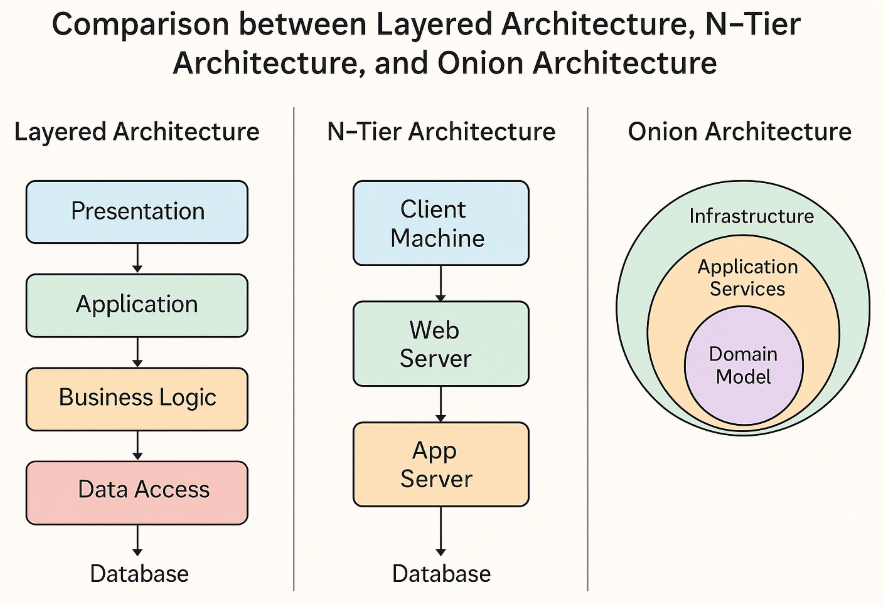
\includegraphics[width=.85\textwidth]{layered_architectures.png}}
  \caption{Une architecture en couches}\label{fig:example}
\end{figure}

\section*{Conclusion}

Suspendisse sit amet nisi placerat, vestibulum nisl vel, iaculis nunc.
Suspendisse quis libero vel ipsum gravida congue nec id arcu. Donec vel mi
viverra, commodo urna vitae, tincidunt lectus. Fusce pellentesque, lectus a
placerat vestibulum, magna lectus placerat nibh, vehicula pellentesque lacus
erat non nulla. Suspendisse maximus, turpis at suscipit egestas, libero massa
ultrices libero, at tincidunt velit eros a eros. Maecenas id tempor nunc.
Phasellus condimentum porttitor sapien in sagittis. Proin in metus diam. Mauris
in turpis sed ex viverra iaculis. Sed lobortis, tellus vitae congue blandit, leo
elit auctor libero, id tempor ante dolor quis quam. Donec eget ligula quam.
Maecenas porttitor massa vel felis elementum tristique.

%------------------------------------------------------------------------------
%	BIBLIOGRAPHY
%------------------------------------------------------------------------------

\nocite{*}
\bibliographystyle{plain}
\bibliography{bibliography}

%------------------------------------------------------------------------------
% BACK MATTER
%------------------------------------------------------------------------------
\appendix

\section{Section en annexe}

Lorem ipsum dolor sit amet, consectetur adipiscing elit. Sed do eiusmod tempor
incididunt ut labore et dolore magna aliqua. Ut enim ad minim veniam, quis
nostrud exercitation ullamco laboris nisi ut aliquip ex ea commodo consequat.
Duis aute irure dolor in reprehenderit in voluptate velit esse cillum dolore eu
fugiat nulla pariatur. Excepteur sint occaecat cupidatat non proident, sunt in
culpa qui officia deserunt mollit anim id est laborum.

\end{document}
